%%%%%%%%%%%%%%%%%%%%%%%%%%%%%%%%%%%%%%%%%%%%%%
%                                            %
%   W Z O R Z E C   S P R A W O Z D A N I A  %
%                                            %
%%%%%%%%%%%%%%%%%%%%%%%%%%%%%%%%%%%%%%%%%%%%%%

% !TeX spellcheck = en_EN
\documentclass[12pt,a4paper]{article}

\usepackage{amsmath,amssymb}
\usepackage[utf8]{inputenc}                                      
\usepackage[OT4]{fontenc}      
%\usepackage[T1]{fontenc}    
%\usepackage{polski}                                                 
\usepackage{indentfirst} 
\usepackage[dvips]{graphicx}
\usepackage{tabularx}
\usepackage{color}
\usepackage{float}
\usepackage{hyperref} 
\usepackage{fancyhdr}
\usepackage{listings}
\usepackage{booktabs}
\usepackage{ifpdf}
\usepackage{mathtext} % polskie znaki w trybie matematycznym
%\makeindex  % utworzenie skorowidza (w dokumencie pdf)
\usepackage{lmodern}
%\usepackage[osf]{libertine}
\usepackage{filecontents}
\usepackage{bchart}
\usepackage{caption,subcaption}
\usepackage{inputenc}

\usepackage{tikz}
\usetikzlibrary{arrows}


\newcounter{nextYear}
\setcounter{nextYear}{\the\year}
\stepcounter{nextYear}

% rozszerzenie nieco strony
%\setlength{\topmargin}{-1cm} \setlength{\textheight}{24.5cm}
%\setlength{\textwidth}{17cm} \addtolength{\hoffset}{-1.5cm}
%\setlength{\parindent}{0.5cm} \setlength{\footskip}{2cm}
%\linespread{1.2} % odstep pomiedzy wierszami

\ifpdf
\DeclareGraphicsRule{*}{mps}{*}{}
\fi


\newcommand{\tl}[1]{\textbf{#1}} 
\pagestyle{fancy}
\renewcommand{\sectionmark}[1]{\markright{\thesection\ #1}}
\fancyhf{} % usuwanie bieżących ustawień
\fancyhead[LE,RO]{\small\bfseries\thepage}
\fancyhead[LO]{\small\bfseries\rightmark}
\fancyhead[RE]{\small\bfseries\leftmark}
\renewcommand{\headrulewidth}{0.5pt}
\renewcommand{\footrulewidth}{0pt}
\addtolength{\headheight}{0.5pt} % pionowy odstęp na kreskę
\fancypagestyle{plain}{%
\fancyhead{} % usuń p. górne na stronach pozbawionych numeracji
\renewcommand{\headrulewidth}{0pt} % pozioma kreska
}

% ustawienia listingu programow
%\lstset{	language=C++, 
%        	numbers=left, 
%        	numberstyle=\tiny, 
%        	stepnumber=1, 
%        	numbersep=5pt,
%		  	stringstyle=\ttfamily,
%			showstringspaces=false,
% 			tabsize=4
%		}

\lstset{%
language=C++,%
commentstyle=\textit,%
identifierstyle=\textsf,%
keywordstyle=\sffamily\bfseries, %
%captionpos=b,%
tabsize=3,%
frame=lines,%
numbers=left,%
numberstyle=\tiny,%
numbersep=5pt,%
breaklines=true,%
morekeywords={Student,Reg,Mark,string},%
escapeinside={(*@}{@*)},%
%basicstyle=\footnotesize,%
%keywords={double,int,for,if,return,vector,matrix,void,public,class,string,%
%float,sizeof,char,FILE,while,do,const}
}
%%%%%%%%%%%%%%%%%%%%%%%%%%%%%%%%%%%%%%%%%%%%%%%%%%%%%%%%%%%%%%%%%%%%%%%

% mala zmiana sposobu wyswietlania notek bocznych
\let\oldmarginpar\marginpar
\renewcommand\marginpar[1]{%
  {\linespread{0.85}\normalfont\scriptsize%
%   \oldmarginpar[\vspace{-1.5ex}\raggedleft\scriptsize\color{black}\textsf{#1}]%    left pages
%                {\vspace{-1.5ex}\raggedright\scriptsize\color{black}\textsf{#1}}% right pades
\oldmarginpar[\hspace{1cm}\begin{minipage}{3cm}\raggedleft\scriptsize\color{black}\textsf{#1}\end{minipage}]%    left pages
{\hspace{0cm}\begin{minipage}{3cm}\raggedright\scriptsize\color{black}\textsf{#1}\end{minipage}}% right pages
}%
}
% % % % % % % % % % % % % % % % % % % % % % % % % % % % % % % %

\begin{document}
\frenchspacing
\thispagestyle{empty}
\begin{center}
{\Large\sf Silesian University of Technology   % Alma Mater

Institute of Informatics

}

\vfill


\includegraphics[width=0.30\textwidth]{images/polsl}

\vfill\vfill

{\Huge\sffamily\bfseries Biologically Inspired Artificial Iintelligence} \\ % tu podać nazwę przedmiotu

\vfill\vfill

{\LARGE\sf Program for lossy compressing images with implementation of self-organizng map(Kohonen SOM)}  % a tu temat laborki :-)


\vfill \vfill\vfill\vfill

%%%%%%%%%%%%%%%%%%%%%%%%%%%%


\begin{tabular}{ll}
\toprule
	author                 						   & Marek Żabiałowicz\\
		e-mail                 						   & marekzabialowicz@gmail.com\\	
	teacher                                             & D.E. Grzegorz Baron			\\
	academic year                                         & 2018/2019					 \\
	study type                                         & SSI					 \\
	major                                               & Computer Science             \\
	semester                                                & 6                           \\
	group                                                  & GkiO4                        \\
	section                                                 & 9                           \\  
	github                                                 & https://github.com/marqustd/ImageSOMCompressorCSharp                           \\  
\bottomrule &  \\
\end{tabular}

\end{center}
%%%%%%%%%%%%%
%%%%%%%%%%%%%%%%%%%%%%%%%%%%%%%%%%%%%%%%%%%%%%%%%%%%%%%%%%%%%%%%%%%%%%%%%
\cleardoublepage
%%%%%%%%%%%%%%%%%%%%%%%%%%%%%%%%%%%%%%%%%%%%%%%%%%%%%%%%%%%%%%%%%%%%%%%%%

%%%%%%%%%%%%%%%%%%%%%%%%%%%%%%%%%%%%%%%%%%%%%%%%%%%%%%%%%%%%%%%%%%%%%%%%%
\section{Introduction}
The aim of my project was to write a program for lossy compresing images with implementation of self-organizng map(Kohonen SOM) with implementaion one or a couple of alghoritims: Winner Takes All, Winner takes Most, Soft Competition Scheme, Stochastic Relaxation, Neuron Gas.

\section{External specification}
The program uses graphical window. With usage of buttons and sliders user can upload an image, set up lattice width and height, compress the image and save it.

\begin{figure}[H]
\centering
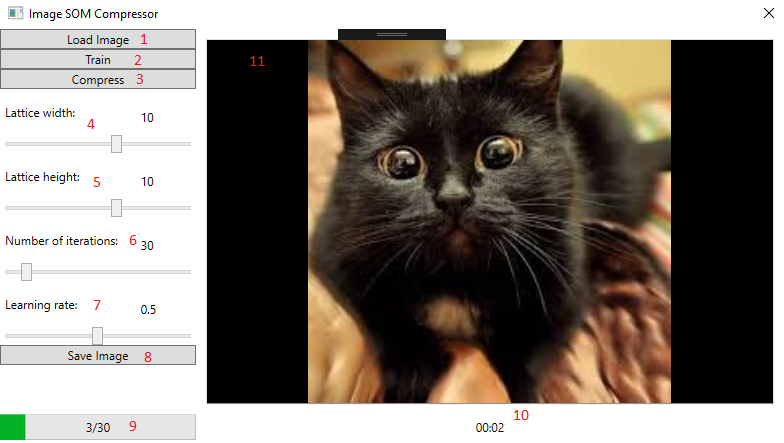
\includegraphics[width=\textwidth]{images/userInterface}
\caption{User interface}
\end{figure}

1 - load the image\\
2 - train self-organizng map\\
3 - compress the image\\
4 - setting latice width\\
5 - setting lattice height\\
6 - setting number of iterations\\
7 - setting a learning rate\\
8 - save the image\\
9 - progeress bar with number of current iteration\\
10 - elapsed time to learn\\
11 - preview of the image(before and after compressing)\\

\section{Internal specification}
The first step in the learning process of self-organizing map is the initialization of all weights(three because of 3 colors RGB) on connections. After that, a first pixel from a picture is used as an input to the network. The network then calculates weights of which neuron are most like the input data (input vector). For this purpose, this formula is used:
\[Distance^2 = \sum_{i=0}^{n} (input_i - weight_i) \]
where n is the number of connection (weights). The map neuron with the best result is called Best Matching Unit or BMU. In an essence, this means that the pixel can be simpled to this neuron.

This means that weights on this connection are updated in a manner that calculated distance is even smaller.

The weights of neighbors of BMU are also modified so they are closer to this pixel too. This is how the whole map is ‘pulled’ toward this point. For this purpose, we have to know the radius of the neighbors that will be updated. This radius is initially large, but it is reduced in every iteration (epoch). The next step in training self-organizing maps is actually calculating mentioned radius value. Following formula is applied:
\[ \sigma(t) = \sigma_0e^{\frac{t}{\lambda}} \]
where t is the current iteration, $\sigma_0$ is the radius of the map. The $\lambda$ in the formula is defined like this:
\[ \lambda=\frac{k}{\sigma_0} \]
where k is the number of iterations. This formula utilizes exponential decay, making radius smaller as the training goes on, which was the initial goal.

When the radius of the current iteration is calculated weights of all neurons within the radius are updated. The closer the neuron is to the BMU the more its weights are changed. This is achieved by using this formula:
\[ weight(t+1)=weight(t)+\Theta(t)L(t)(input(t)-weight(t)) \]

This is the main learning formula, and it has a few important points that should be discussed. The first one is L(t) which represents the learning rate. Similarly to the radius formula, it is utilizing exponential decay and it is getting smaller in every iteration:
\[ L(t)=L_0e^{-\frac{t}{\lambda}} \]
Apart from that, we mentioned that the weight of the neuron will be more modified if that neuron is closer to the BMU. In the formula, that is handled with the $\Theta(t)$. This value is calculated like this:
\[ \Theta(t)=e^{-distBMU/2\sigma(t)^2} \]

The whole alghoritim we can write in 7 steps:\\
1. Weight initialization.\\
2. The pixel is selected from the picture and used as an input for the network.\\
3. BMU is calculated.\\
4. The radius of neighbors that will be updated is calculated.\\
5. Each weight of the neurons within the radius are adjusted to make them more like the input vector.\\
6. Steps from 2 to 5 are repeated for each input vector of the dataset.\\
7. Steps from 2 to 6 are repeated till the end.

But after simpilying picture to 256 pixels(lattice 16x16) we need to save the picture. 

\begin{lstlisting}

private void SaveToFile(string filename, SomFileModel model)
        {
            using (var outputFile = new BinaryWriter(new FileStream(filename, FileMode.OpenOrCreate)))
            {
                outputFile.Write((byte) (model.Neurons.Count - 1));
                foreach (var neuron in model.Neurons)
                {
                    outputFile.Write(neuron.R);
                    outputFile.Write(neuron.G);
                    outputFile.Write(neuron.B);
                }

                outputFile.Write(model.Width);
                outputFile.Write(model.Height);

                var former = model.Input[0];
                byte count = 0;

                for (var i = 0; i < model.Input.Count; i++)
                {
                    if (model.Input[i] == former && count < byte.MaxValue)
                    {
                        count++;

                        if (i == model.Input.Count - 1)
                        {
                            outputFile.Write(former);
                            outputFile.Write(count);
                        }
                    }
                    else
                    {
                        outputFile.Write(former);
                        outputFile.Write(count);

                        former = model.Input[i];
                        count = 1;
                    }
                }
            }
        }
\end{lstlisting}

Firstly I write a number of neurons, then describe all neurons each with 3 bytes, each byte for one color(RGB). Next I write picture's width and height and all pixels in format [neuron index|number].

\section{Testing the program}
I've tested the program with 3 kind of files - small(255x255), big(400x400) and cartoon and several setups. 
    
\begin{figure}[H]
    \centering % <-- added
\begin{subfigure}{0.25\textwidth}
  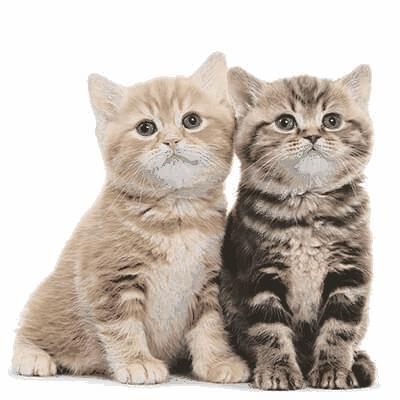
\includegraphics[width=\linewidth]{images/big/original}
  \caption{original}
  \label{fig:1}
\end{subfigure}\hfil % <-- added
\begin{subfigure}{0.25\textwidth}
  
\includegraphics[width=\linewidth]{images/big/3-3-5-05}
  \caption{3x3 5 0.5}
  \label{fig:2}
\end{subfigure}\hfil % <-- added
\begin{subfigure}{0.25\textwidth}
  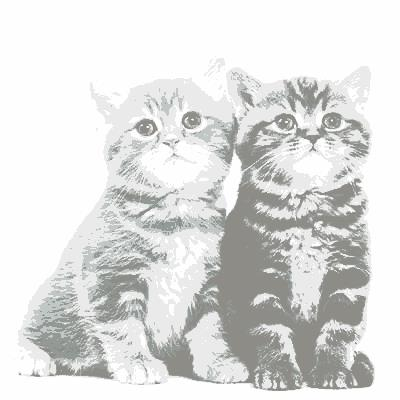
\includegraphics[width=\linewidth]{images/big/3-3-30-05}
  \caption{3x3 30 0.5}
  \label{fig:3}
\end{subfigure}

\medskip
\begin{subfigure}{0.25\textwidth}
  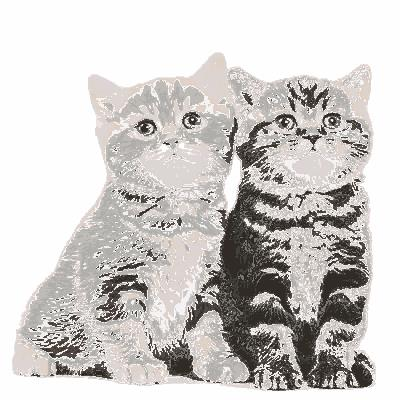
\includegraphics[width=\linewidth]{images/big/5-5-50-001}
  \caption{5x5 50 0.01}
  \label{fig:4}
\end{subfigure}\hfil % <-- added
\begin{subfigure}{0.25\textwidth}
  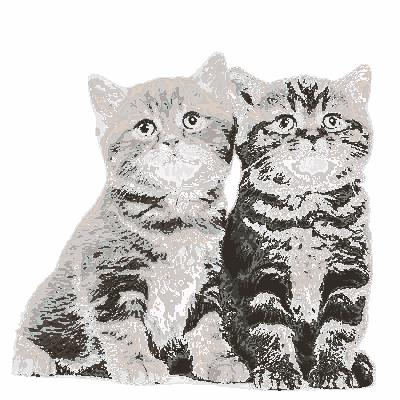
\includegraphics[width=\linewidth]{images/big/5-5-255-05}
  \caption{5x5 255 0.5}
  \label{fig:5}
\end{subfigure}
\begin{subfigure}{0.25\textwidth}
  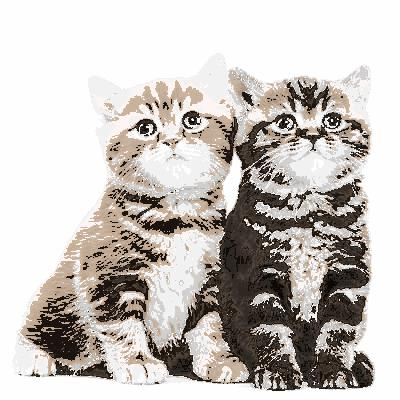
\includegraphics[width=\linewidth]{images/big/6-6-30-05}
  \caption{6x6 30 0.5}
  \label{fig:6}
\end{subfigure}\hfil % <-- added

\medskip
\begin{subfigure}{0.25\textwidth}
  
\includegraphics[width=\linewidth]{images/big/12-12-30-05}
  \caption{12x12 30 0.5}
  \label{fig:6}
\end{subfigure}
\begin{subfigure}{0.25\textwidth}
  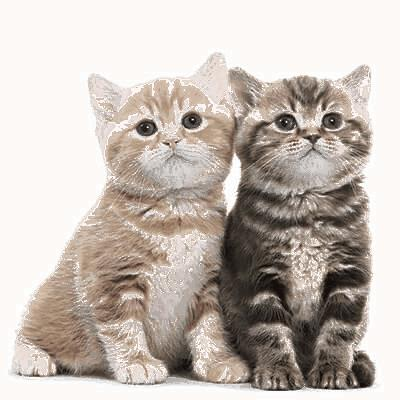
\includegraphics[width=\linewidth]{images/big/16-16-30-05}
  \caption{16x16 30 0.5}
  \label{fig:4}
\end{subfigure}\hfil % <-- added
\begin{subfigure}{0.25\textwidth}
  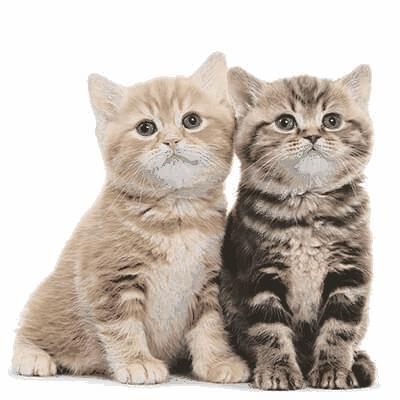
\includegraphics[width=\linewidth]{images/big/16-16-50-001}
  \caption{16x16 50 0.01}
  \label{fig:5}
\end{subfigure}\hfil % <-- added

\medskip
\begin{subfigure}{0.25\textwidth}
  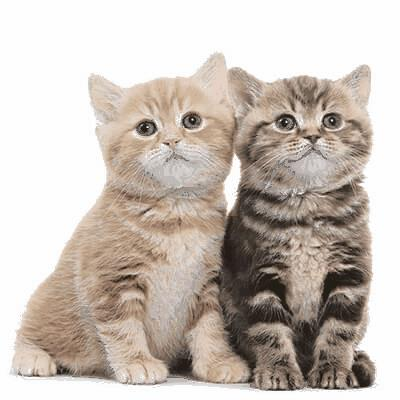
\includegraphics[width=\linewidth]{images/big/16-16-50-1}
  \caption{16x16 50 1}
  \label{fig:4}
\end{subfigure}\hfil % <-- added
\begin{subfigure}{0.25\textwidth}
  
\includegraphics[width=\linewidth]{images/big/16-16-100-05}
  \caption{16x16 100 0.5}
  \label{fig:6}
\end{subfigure}
\begin{subfigure}{0.25\textwidth}
  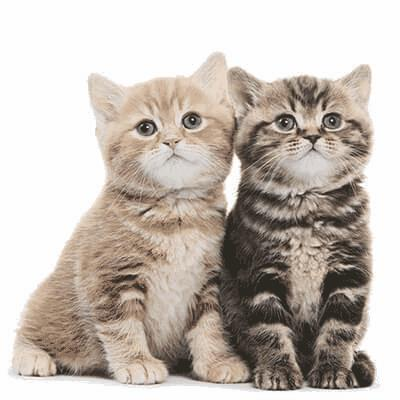
\includegraphics[width=\linewidth]{images/big/16-16-255-05}
  \caption{16x16 255 0.5}
  \label{fig:5}
\end{subfigure}\hfil % <-- added


\caption{big picture - 400x400}
\label{fig:images}
\end{figure}

\begin{figure}[H]
    \begin{bchart}[max=500]
        \bcbar[text=original]{469}
            \smallskip
        \bcbar[text=jpg]{25.3}
            \smallskip
        \bcbar[text=b]{18.7}
            \smallskip
        \bcbar[text=c]{60.4}
            \smallskip
        \bcbar[text=d]{105}
            \smallskip
        \bcbar[text=e]{110}
            \smallskip
        \bcbar[text=f]{108}
            \smallskip
        \bcbar[text=g]{143}
            \smallskip
        \bcbar[text=h]{156}
            \smallskip
        \bcbar[text=i]{162}
            \smallskip
        \bcbar[text=j]{160}
            \smallskip
        \bcbar[text=k]{162}
            \smallskip
        \bcbar[text=l]{161}
    \end{bchart}
    \caption{Diference in size in big picture files in kB}
    \end{figure}
    
    We can see that there's a huge difference between first 5 pictures and the other ones in Fig.2. The quality has improved but also the size of files has increased(Fig.3). Last row is almost the same as original file.
    
\begin{figure}[H]
    \centering % <-- added
\begin{subfigure}{0.25\textwidth}
  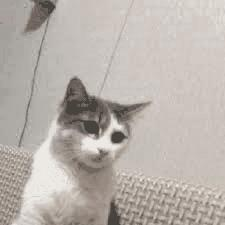
\includegraphics[width=\linewidth]{images/small/original}
  \caption{original}
  \label{fig:1}
\end{subfigure}\hfil % <-- added
\begin{subfigure}{0.25\textwidth}
  
\includegraphics[width=\linewidth]{images/small/3-3-5-05}
  \caption{3x3 5 0.5}
  \label{fig:2}
\end{subfigure}\hfil % <-- added
\begin{subfigure}{0.25\textwidth}
  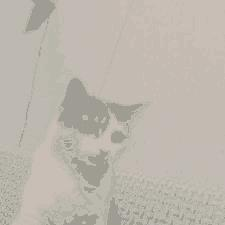
\includegraphics[width=\linewidth]{images/small/3-3-30-05}
  \caption{3x3 30 0.5}
  \label{fig:3}
\end{subfigure}

\medskip
\begin{subfigure}{0.25\textwidth}
  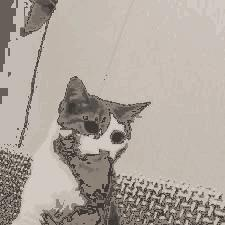
\includegraphics[width=\linewidth]{images/small/5-5-50-001}
  \caption{5x5 50 0.01}
  \label{fig:4}
\end{subfigure}\hfil % <-- added
\begin{subfigure}{0.25\textwidth}
  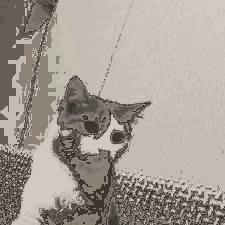
\includegraphics[width=\linewidth]{images/small/5-5-255-05}
  \caption{5x5 255 0.5}
  \label{fig:5}
\end{subfigure}\hfil % <-- added
\begin{subfigure}{0.25\textwidth}
  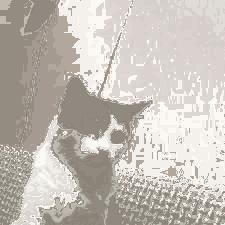
\includegraphics[width=\linewidth]{images/small/6-6-30-05}
  \caption{6x6 30 0.5}
  \label{fig:6}
\end{subfigure}

\medskip
\begin{subfigure}{0.25\textwidth}
  
\includegraphics[width=\linewidth]{images/small/12-12-30-05}
  \caption{12x12 30 0.5}
  \label{fig:6}
\end{subfigure}\hfil % <-- added
\begin{subfigure}{0.25\textwidth}
  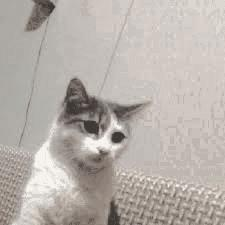
\includegraphics[width=\linewidth]{images/small/16-16-30-05}
  \caption{16x16 30 0.5}
  \label{fig:4}
\end{subfigure}\hfil % <-- added
\begin{subfigure}{0.25\textwidth}
  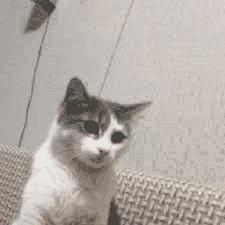
\includegraphics[width=\linewidth]{images/small/16-16-50-001}
  \caption{16x16 50 0.01}
  \label{fig:5}
\end{subfigure}

\medskip
\begin{subfigure}{0.25\textwidth}
  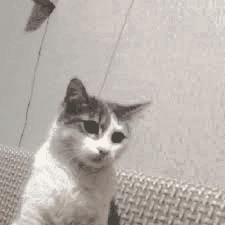
\includegraphics[width=\linewidth]{images/small/16-16-50-1}
  \caption{16x16 50 1}
  \label{fig:4}
\end{subfigure}\hfil % <-- added
\begin{subfigure}{0.25\textwidth}
  
\includegraphics[width=\linewidth]{images/small/16-16-100-05}
  \caption{16x16 100 0.5}
  \label{fig:6}
\end{subfigure}\hfil % <-- added
\begin{subfigure}{0.25\textwidth}
  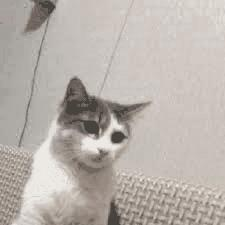
\includegraphics[width=\linewidth]{images/small/16-16-255-05}
  \caption{16x16 255 0.5}
  \label{fig:5}
\end{subfigure}


\caption{small picture - 255x255}
\label{fig:images}
\end{figure}

\begin{figure}[H]
    \begin{bchart}[max=150]
        \bcbar[text=original]{148}
            \smallskip
        \bcbar[text=jpg]{4.23}
            \smallskip
        \bcbar[text=b]{22.8}
            \smallskip
        \bcbar[text=c]{24.2}
            \smallskip
        \bcbar[text=d]{36}
            \smallskip
        \bcbar[text=e]{37}
            \smallskip
        \bcbar[text=f]{36.3}
            \smallskip
        \bcbar[text=g]{55.3}
            \smallskip
        \bcbar[text=h]{61.3}
            \smallskip
        \bcbar[text=i]{61.2}
            \smallskip
        \bcbar[text=j]{60.8}
            \smallskip
        \bcbar[text=k]{60.6}
            \smallskip
        \bcbar[text=l]{60.9}
    \end{bchart}    
        \caption{Diference in size in small picture files in kB}
    \end{figure}
    
    \begin{figure}[H]
    \centering % <-- added
\begin{subfigure}{0.25\textwidth}
  
\includegraphics[width=\linewidth]{images/cartoon/original}
  \caption{original}
  \label{fig:1}
\end{subfigure}\hfil % <-- added
\begin{subfigure}{0.25\textwidth}
  
\includegraphics[width=\linewidth]{images/cartoon/3-3-5-05}
  \caption{3x3 5 0.5}
  \label{fig:2}
\end{subfigure}\hfil % <-- added
\begin{subfigure}{0.25\textwidth}
  
\includegraphics[width=\linewidth]{images/cartoon/3-3-30-05}
  \caption{3x3 30 0.5}
  \label{fig:3}
\end{subfigure}

\medskip
\begin{subfigure}{0.25\textwidth}
  
\includegraphics[width=\linewidth]{images/cartoon/5-5-50-001}
  \caption{5x5 50 0.01}
  \label{fig:4}
\end{subfigure}\hfil % <-- added
\begin{subfigure}{0.25\textwidth}
  
\includegraphics[width=\linewidth]{images/cartoon/5-5-255-05}
  \caption{5x5 255 0.5}
  \label{fig:5}
\end{subfigure}\hfil % <-- added
\begin{subfigure}{0.25\textwidth}
  
\includegraphics[width=\linewidth]{images/cartoon/6-6-30-05}
  \caption{6x6 30 0.5}
  \label{fig:6}
\end{subfigure}

\medskip
\begin{subfigure}{0.25\textwidth}
  
\includegraphics[width=\linewidth]{images/cartoon/12-12-30-05}
  \caption{12x12 30 0.5}
  \label{fig:7}
\end{subfigure}\hfil % <-- added
\begin{subfigure}{0.25\textwidth}
  
\includegraphics[width=\linewidth]{images/cartoon/16-16-30-05}
  \caption{16x16 30 0.5}
  \label{fig:8}
\end{subfigure}\hfil % <-- added
\begin{subfigure}{0.25\textwidth}
  
\includegraphics[width=\linewidth]{images/cartoon/16-16-50-001}
  \caption{16x16 50 0.01}
  \label{fig:9}
\end{subfigure}

\medskip
\begin{subfigure}{0.25\textwidth}
  
\includegraphics[width=\linewidth]{images/cartoon/16-16-50-1}
  \caption{16x16 50 1}
  \label{fig:10}
\end{subfigure}\hfil % <-- added
\begin{subfigure}{0.25\textwidth}
  
\includegraphics[width=\linewidth]{images/cartoon/16-16-100-05}
  \caption{16x16 100 0.5}
  \label{fig:11}
\end{subfigure}\hfil % <-- added
\begin{subfigure}{0.25\textwidth}
  
\includegraphics[width=\linewidth]{images/cartoon/16-16-255-05}
  \caption{16x16 255 0.5}
  \label{fig:12}
\end{subfigure}


\caption{cartoon picture}
\label{fig:images}
\end{figure}

\begin{figure}[H]
    \begin{bchart}[max=200]
        \bcbar[text=original]{192}
            \smallskip
        \bcbar[text=jpg]{13.1}
            \smallskip
        \bcbar[text=b]{23.9}
            \smallskip
        \bcbar[text=c]{13.9}
            \smallskip
        \bcbar[text=d]{32.5}
            \smallskip
        \bcbar[text=e]{31.7}
            \smallskip
        \bcbar[text=f]{36.1}
            \smallskip
        \bcbar[text=g]{49}
            \smallskip
        \bcbar[text=h]{56.5}
            \smallskip
        \bcbar[text=i]{57.9}
            \smallskip
        \bcbar[text=j]{58.4}
            \smallskip
        \bcbar[text=k]{58.2}
            \smallskip
        \bcbar[text=l]{57.8}
    \end{bchart} 
            \caption{Diference in size in cartoon picture files in kB}
    \end{figure}
The same situation we can see in a small file and cartoon(Fig.4 and Fig.6). There is a visible difference between second and third row.

The best improvement in quality is made by increasing the lattice size. Incresing number of iterations increases contrast of the image. Changing learing rate seems to have no impact.

I managed only once to create a file lower than jpg, but the quality is a lot worse.

\section{Further remarks}
The self-organizing map alghoritim should be implemented with usage of GPU and CUDA. I developed a code in C\# and currently, there is no fully supported way to create a program for GPU with .NET. I tried to use library Hybrydizer, but after a couple days Igave up.

The proper way is to implement alghoritim in C++ and then with usage NSight and CUDA made it for GPU.
\section{Conclusions}
Taking into consideration size of compressed pictures, their quality and also time needed to compress one image, my alghorithm will not revolutionize image proccessing industry. But the project thought me principals behind using a self-organizing kohonen map.

I also learned that it's better to not use high-level programming laungage such as C\# to implement artificial iintelligence.
\end{document}
% Koniec wieńczy dzieło.
